% 
% Annual Cognitive Science Conference
% LaTeX Paper -- Proceedings Format
% 

% Original : Jin-Hwa Kim (jhkim@bi.snu.ac.kr)        06/02/2014
% Modified : Jin-Hwa Kim (jhkim@bi.snu.ac.kr)        06/22/2014

%% Change ``a4paper'' in the following line to ``letterpaper'' if you are
%% producing a letter-format document.

\documentclass[10pt,letterpaper]{article}

\usepackage{cogsci}
\usepackage{pslatex}
\usepackage{apacite}

\usepackage{nameref}
\usepackage{graphicx}
\usepackage{subfigure}

\title{Active Long Fixation Correlates with the Formation of\\
Long-Term Memory}
 
\author{{\large \bf Jin-Hwa Kim (jhkim@bi.snu.ac.kr)} \\
  Interdisciplinary Program in Cognitive Science, Seoul National University \\
  Seoul, 151-742, Republic of Korea
  \AND {\large \bf Byoung-Tak Zhang (btzhang@bi.snu.ac.kr)} \\
  School of Computer Science and Engineering, Seoul National University \\
  Seoul, 151-742, Republic of Korea}

\begin{document}

\maketitle

\begin{abstract}
The application of eyewear accelerates the study on the eye movement, for the eye movement is a non-invasive and convenient indicator of the brain activities. We investigate the eye movements of the subjects watching the kids video. First, we conduct the long-term memory test of whether fixation duration correlates with long-term memory. Second, we classify its visual constraints into alert and no alert types. As a result of the test, the fixation duration itself is not decisive. However, the long fixations which are actively engaged with alert type movie clips statistically have higher scores, while the short fixations do not. Finally, we propose a simple computational model using the linear regression of two significant features, saliency scrutiny and fixation duration. It may provide an explanatory way to the efficient memory mechanism for the life-long sequences.

\textbf{Keywords:} 
Human Factors and Human-computer interaction; Cognitive Science; Memory; Statistics; Event cognition; Eye tracking
\end{abstract}



\section{Introduction}

The visual information is easily affected by the moment-to-moment environmental changes, heuristic but robust compensation strategies are required. Hence, how the brain processes the visual information provides the profound way to study the mechanism by which the brain precisely and efficiently processes the most dynamic and enormous sensory information.

There are a lot of studies on the computational modeling for the visual information, which include the visual fragment completion, the scene or object classification and recognition, and object tracking. These research topics often tend to focus on the objective for each task, not on the implementation of the method how the brain deals with the visual information. As a result, the computational approach to the modeling for the visual information processing of the brain is gradually changed to the optimization problem, which hinders the understandings of the human-level information processing abilities. 

Particularly, the object tracking seems to describe how we pay attention to an interesting object, however, the eye movement, mostly controlled by the oculomotor system, complicates with how the brain works for the acquisition of the visual information \cite{Henderson2003}. For instance, in the fixation state, the human eyes only recognize the small portion of the whole sight. If you read this paper from an 8-inch distance fixing on one particular letter, you cannot read outside of next two words or about ten letters which are presented in the para-fovea. Since the brain is well-known for its parallel processing on the neural circuits, this sequential notion of eye movement for the visual system would be inefficient for information processing. Therefore, we should notice that the experimental results of covert attention and shifting receptive field are also the important subject to study \cite{Zirnsak2014}.

The studies on the reading eye movement, which are relatively well studied by psychologists and neuroscientists, reveal that fixation duration is related to the presence of the cognitive process, such as observing its correlation with linguistic attributes \cite{Inhoff1986,Rayner1986}.

We investigate the characteristics of eye movements on the video stimuli focusing on the formation of long-term memory using recognition test. In this study, we focus on the characteristics of the fixation duration as the evidence of the cognitive process to memorize. Moreover, as the movie clips which potentially induce emotional arousal are known to increase the recognition of the previously watched movie clips \cite{Cahill1996amyg,Cahill1998baso}, we will see if the arousal effect is asserted by the duration of fixation. Finally, we propose a linear regression model based on the active features of eye movement, saliency scrutiny and fixation duration.



\section{Materials and Methods}
\label{sec:material-and-methods}

For this study, we prepared the video material \textit{Pororo Season 3}, which is a famous kids video in Republic of Korea. In this video, there are artificial 3D-rendered characters and other objects who have distinctive traits, so visual features are easily captured by eye movements. \textit{Pororo Season 3 DVD 1} contains 13 consecutive episodes, each with a different single storyline. The total playing time is 67 minutes and 50 seconds.

We recruited 11 participants with normal vision (6 males, 5 females; 23-31 age), who are graduate students in Seoul National University, voluntarily participated in the study. For the stability of collecting data and the eye gear requires appropriate head circumference, we chose the target participants for this study. All participants had not experienced a brain damage or a behavioral disorder. The participants were first time viewers of the video, \textit{Pororo Season 3}. To prevent distraction, each participant took a set of tests for the two-split video, one is about 32 minutes of the first half and the other is about 36 minutes of the later half, each on the other day. Later then, we merged two parts into one manually, in a way that the results do not overlap. 

Participants watched the kids video in the room which has the experimental settings. The room is about 3 square meters surrounded by the opaque curtains. On the side of the room, a wide-screen HDTV (1920x1080 resolution, 885 mm x 500 mm, 16:9 ratio) was installed, and 2.1 channel speakers. Participants were guided to sit on a comfortable sofa in front of 1.7 m from the TV screen.

Concurrently, the eye movements and the user-perspective scenes were recorded by \textit{Tobii Glasses eye tracker}, the corneal reflection based system with a sampling rate of 30 Hz. We used the \textit{I-VT algorithm} as the fixation filter (system default), which classified fixations with the velocity threshold of 30 degree per second. Usually, the saccadic eye movements are discriminated with low velocities (less than 100 degree/second) and high velocities (higher than 300 degree/second), in which the velocity-based classification is a simple and reasonable approach \cite{Salvucci2000}.

We prepared the controlled memory test for each participant. We conducted this study 3-4 months after the first session of watching (the intervals are not consistent due to schedule conflicts). A memory test consisted of total 20 movie clips; 8 movie clips for long fixations, another 8 movie clips for short fixations, and the remaining 4 movie clips for the control, which were not seen in the previous study. In detail, the lengths of all movie clips were each 3-second long. \textit{The long fixation sequences} were randomly picked from each participant's data containing the fixation longer than 1400 ms in the middle of the movie clip. \textit{The short fixation sequences} were randomly picked from each participant's data containing the fixation shorter than 300 ms. The 4 control movie clips were randomly picked from the other season of \textit{Pororo} series, \textit{Pororo Season 2}.

Each participant identified 20 movie clips that were sorted randomly. Each participant gave a score for each movie clip between 1 and 5, which is an integer, depending on the assurance of whether he or she saw the movie clip before or not. Notice that, in this study, 1 is the lowest score, not 0, which means that the movie clip is surely not seen.



\section{Fixation Duration}
\label{sec:fixation-duration}
\label{subsec:Long-Fixation-Durations}

\begin{figure}[ht]
  \centerline{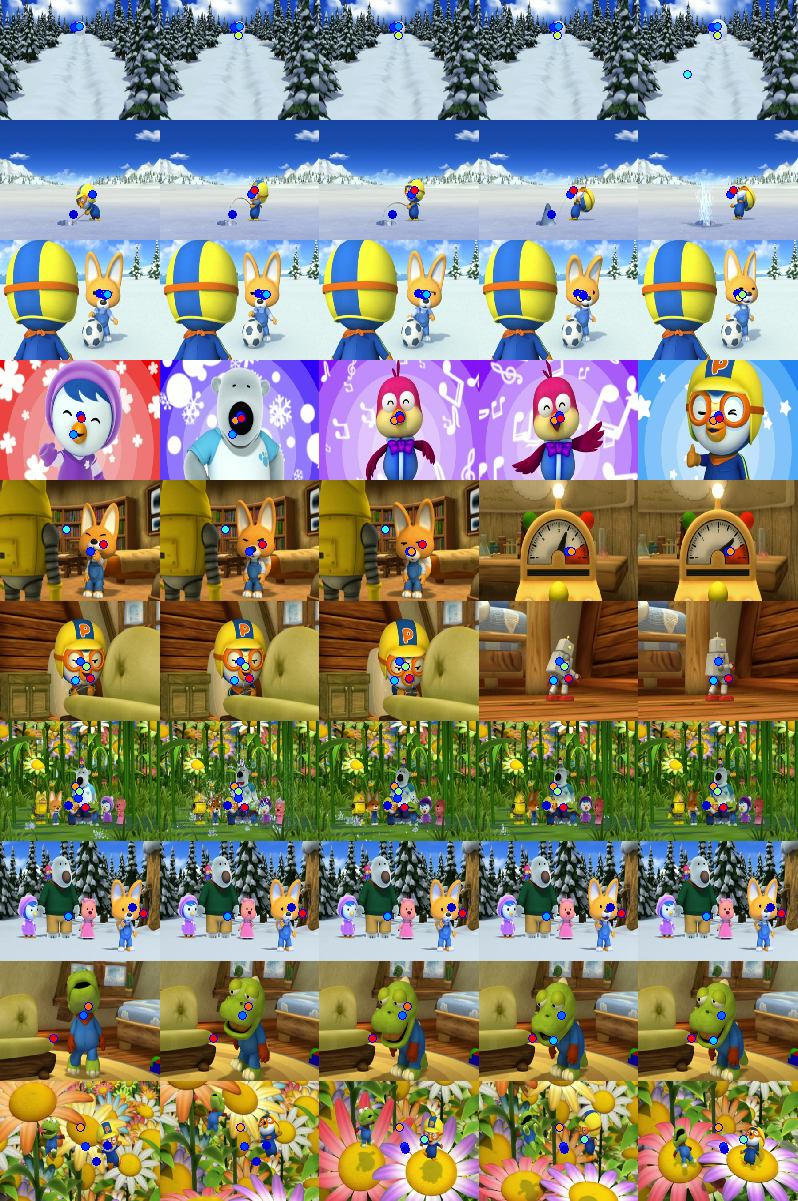
\includegraphics[width=76mm]{./eps/long_fixations_types.png}}
  \caption[The samples of sequence types]{The sequences of frames which received more than 2 seconds of fixation duration from at least 3 participants. First 3 sequences show the \textit{alerted} type, then next 3 sequences show the \textit{successive} type, then next 3 sequences show the \textit{stationary} type, and then the last sequence shows the \textit{unclassified} type of visual constraints for the review. For the description of those sequences, see the text in Section~\textit{\nameref{subsec:Long-Fixation-Durations}}.}
  \label{fig:long-fixations}
\end{figure}

In the video watching task, we anticipated the characteristics of fixation duration to be different from those in the reading task. As expected, the fixation duration was changed more drastically, up to 10 seconds during watching the video. These changes were partly caused by the sequential changes of the visual stimuli and the fluctuated responses of the oculomotor system and cognitive processes.

In Figure~\ref{fig:long-fixations} the sequences of frames which received more than 2 seconds of the fixation duration from at least 3 different participants are shown. We set the threshold to reduce the interpersonal variation. We got all 41 sequences across 1 hour 7 minutes 50 seconds length of the material. For the review, we chose 10 typical sequences. Each row represents an independent sequence and each column shows a single frame. The time interval between the frames is 0.5 seconds. The colored dots represent the fixation positions, whose durations are longer than 2 seconds. The same color means the same participant. Four different types of the sequences are listed as \textit{alerted} (3), \textit{successive} (3), \textit{stationary} (3), and \textit{unclassified} (1) for the review. The classification is conducted by one of authors and two other colleagues. Every sequence used by this study is classified by agreement. If there is a conflict or not fit to the major types, then the sequence is classified as \textit{unclassified}.

The sequence of the \textit{alerted} type was classified because the scene implied an unusual and, potentially dangerous or difficult situation, which may introduce a mental arousal. The sequence of the first row demonstrates an urgent moment that a huge snowball is about to roll down the hill, which was previously rolled up by the robot, \textit{Rody}. Second shows that \textit{Pororo} has been fishing at the ice hole, but what he caught was \textit{Shark}, a naughty character. Third shows that \textit{Eddy} rolled his eyes to kick his ball avoiding the opponent \textit{Pororo}.

The \textit{successive} type shows that the fixation duration extends across more than 2 different scenes. Because the location of the target object is not changed or changed within the range of a foveal or central vision, 2-5$^{\circ}$, the fixation holds its position \cite{mcmorris2014acquisition}. The fourth sequence shows the closed-up characters are serially shown up in the center of the screen. The fixations duration of the fifth and sixth sequences extends across different scenes have different visual configurations.

The \textit{stationary} type most clearly shows the characteristics that the indifferent scene maintains while the target object moves a little bit or even does not move. For there is not a particular event or a change of the scene, the participants tend to fixate their gazes. See the seventh through ninth sequences.

The sequence of the \textit{unclassified} type takes various forms. The tenth sequence shows that \textit{Pororo} and \textit{Crong} just jumped out of the shoulder of the magician dragon \textit{Tongtong}, who is flying in the sky. Two sunflowers spring \textit{Pororo} and \textit{Crong} into the sky in multiple times. 

\begin{figure}[ht]
  \centerline{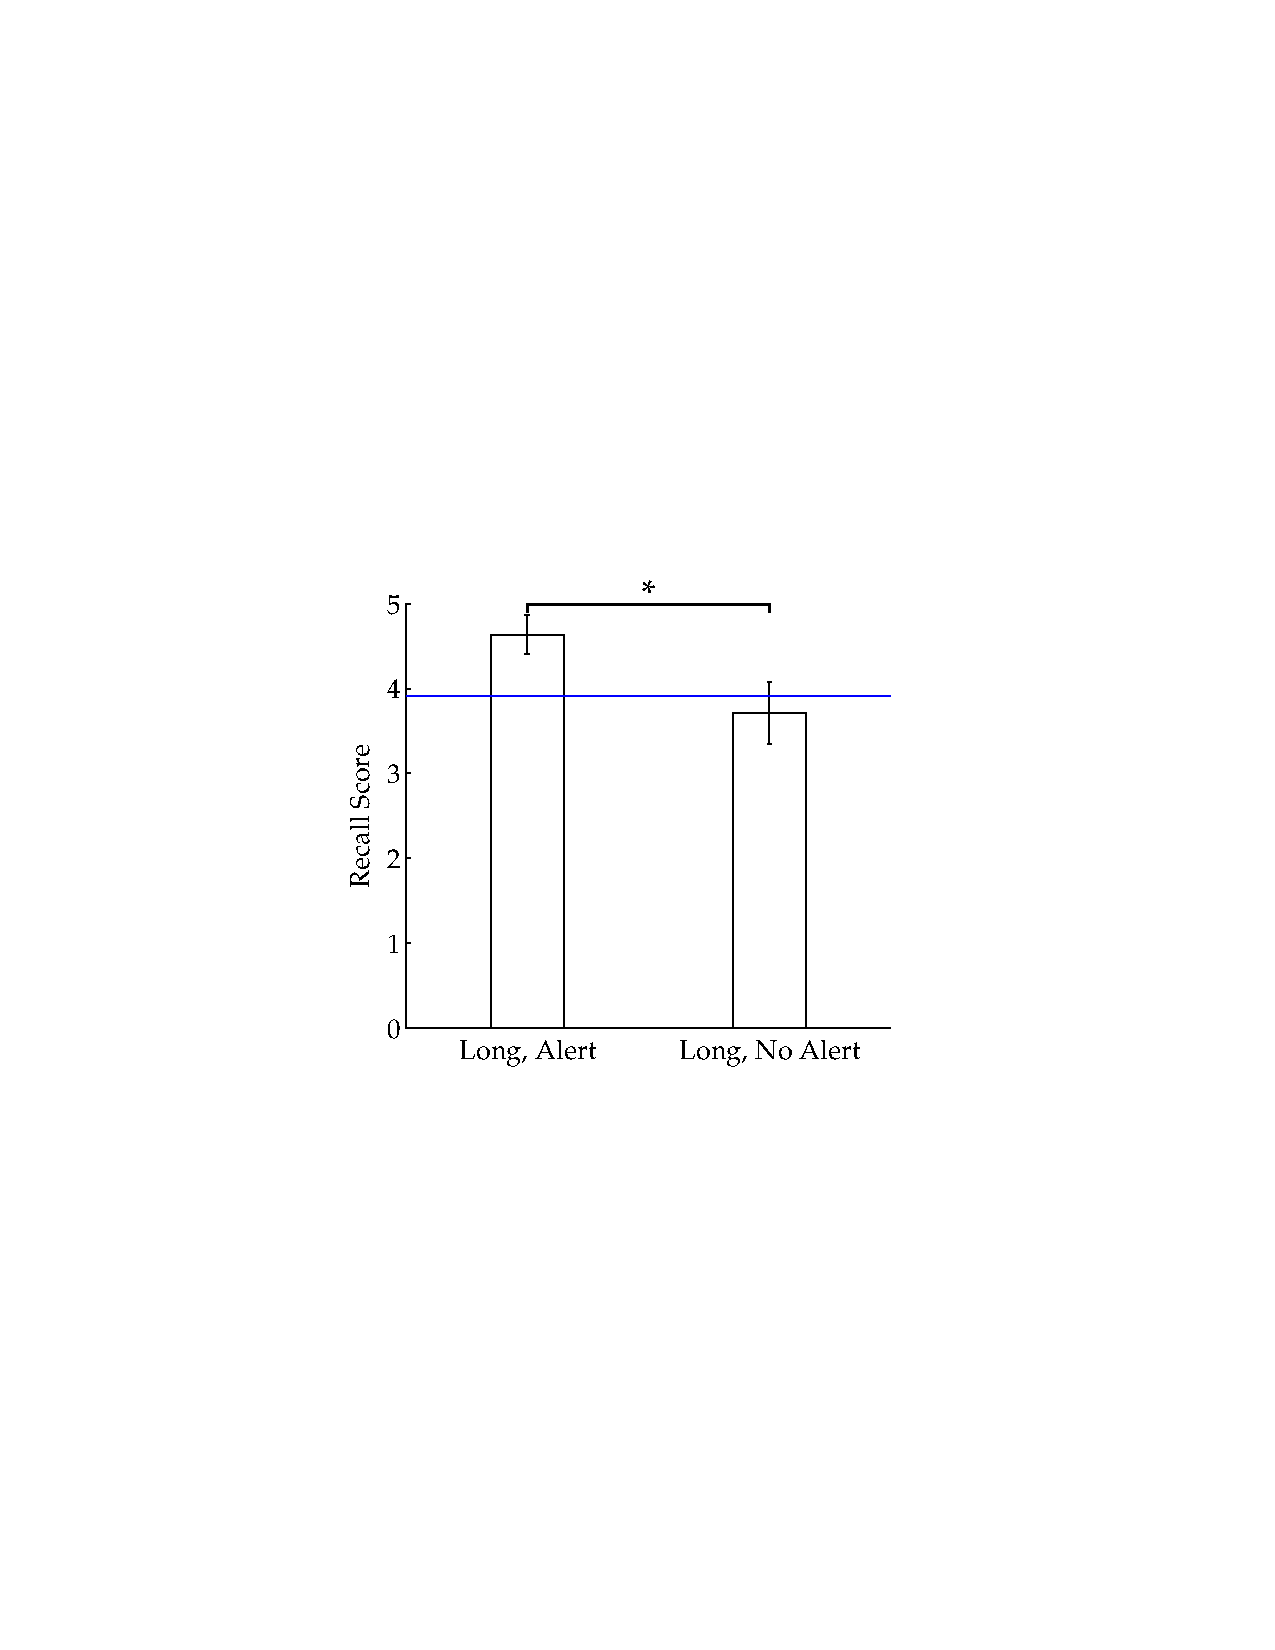
\includegraphics[width=70mm,height=56mm,trim=54mm 100mm 54mm 98mm]{./eps/memtest_long.pdf}}
  \caption[The memory test result for the long fixations which are on alert movie clips or no alert movie clips]{The memory test result for the long fixations which is on the \textit{alert} movie clips or the \textit{no alert} movie clips. The blue horizontal line indicates the mean scores of the long fixated movie clips. Error bars indicate $\pm$ 2 SEMs.}
  \label{fig:memtest-long}
\end{figure}

\begin{figure}[ht]
  \centerline{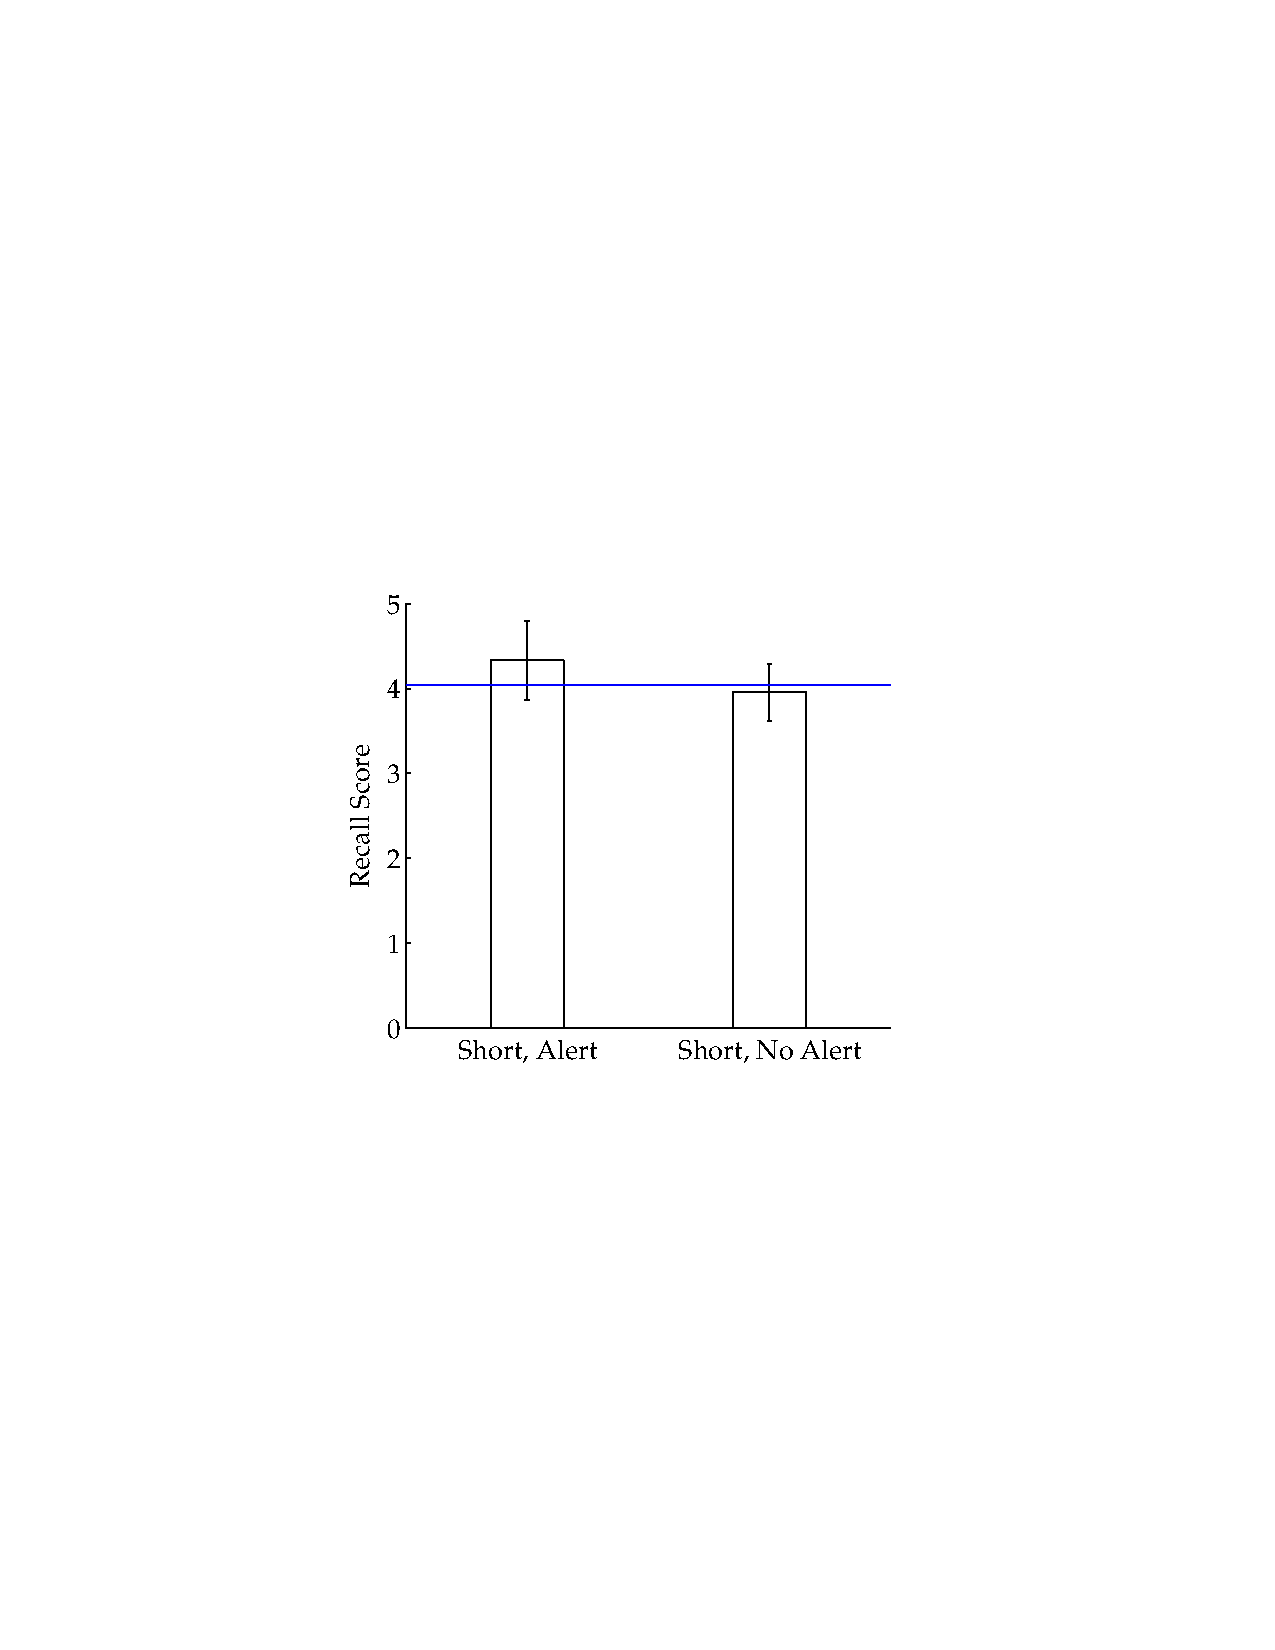
\includegraphics[width=70mm,height=56mm,trim=54mm 100mm 54mm 98mm]{./eps/memtest_short.pdf}}
  \caption[The memory test result for the short fixations which are on the alert movie clips or no alert movie clips]{The memory test result for the short fixations which is on the \textit{alert} movie clips or the \textit{no alert} movie clips.}
  \label{fig:memtest-short}
\end{figure}



\section{Long-Term Memory Formation}

In the studies of reading eye movements, as noted before, the fixation duration is a good indicator for information processing. Even so, when we applied to a watching task, we have to be more cautious that the long fixation itself was not always induced when the internal state of a subject is affected. Furthermore, the sequences that received a long fixation did not decisively guarantee the quality of information processing nor its specificity. When we carefully look into the sequences in Figure~\ref{fig:long-fixations}, the fixations on \textit{successive} or \textit{stationary} type sequences can be interpreted as looking passively or even blankly.

A stimulus is memorized by the constructive activities, which is a series of stimulations, giving attention, and acquisition. Yet the corresponding responses are not deterministic by the stimulus for the uncertainty of environmental perturbations or the complexity of internal states. Therefore, the formation of memory is the result of the cognitive process of response rather than the response itself. We need to discern the reliable indicator of the cognitive process with a sufficient care.


\subsection{Recognition Test}

We defined two types of fixation as long and short fixations. The long fixation was defined by the gaze holding its position after fixation filtering, which is longer than 1400 ms. The short fixation was defined by the one that is shorter than 300 ms. Each participant assessed in a recognition test rating 20 movie clips, containing 8 long fixated movie clips, 8 short fixated movie clips and 4 not-seen movie clips, which were not seen previously. Contrary to our expectations, the scores for the short fixated movie clips were not much different from the scores for the long fixated movie clips (p $=$ 0.5051). This result makes sense considering that the long fixation is an attentive response, which can be actively or passively motivated by a reciprocal process in visual system.

The relationship between the emotional arousal and the formation of long-term memory was known for the studies in neuroscience \cite{Cahill1996amyg,Cahill1998baso}. Although it is not included in this paper, the arousal effect on the recognition test was verified. \textit{Alert} movie clips significantly got higher scores than \textit{no alert} movie clips with the p-value of 0.0077 (p $<$ 0.01). On top of this, more detailed analyses are conducted with regard to this.

Figure~\ref{fig:memtest-long} shows the memory test result for the long fixation which was on the \textit{alert} movie clip or the \textit{no alert} movie clip. The \textit{alert} movie clips included the emotional arousal events, which was previously defined. This classification is rather definite because the content is an animation video for children. The numbers of ratings from 11 participants were 19 for the \textit{alert} and 69 for \textit{no alert}. The difference between the two mean scores for the long and short fixation types was significant. The p-value of two-sample t-test was 0.0104 ($<$ 0.05).

Figure~\ref{fig:memtest-short} shows the memory test result for the short fixation which was on the \textit{alert} movie clips or the \textit{no alert} movie clips. The numbers of cases from 11 participants were 21 and 67, respectively. The p-value of two-sample t-test was 0.2484 ($>$ 0.05). In the short fixation cases, there was no significance between the two content types, \textit{alert} type and \textit{no alert} type.


\subsection{Gaze Variations}
\label{subsec:gaze-variations}

The difference of the eye movements between the \textit{alert} movie clips and the \textit{no alert} movie clips for the long fixated was observed by the variation of gazes. Actually, the gazes keep moving in the fixation state, because eye balls are fixed by twitching extraocular muscles. However, the most contribution to that variation was a smooth pursuit. In the smooth pursuit, the eyes were following a slowly moving object or interesting features. Because our experimental settings did not and can not precisely define the smooth pursuit, all the eye movements slower than 30 degree per second were candidates. 

To get the variation of the gazes excluding the variation from the smooth pursuit, we used the window sliding technique. Varying the size of a time window, we moved the time window on the time series by 1/30 second in every step, and took the median of the variations. Figure~\ref{fig:gaze-variation} shows the significant level changes according to the change of the window size. If the window size was smaller than 200 ms, p-values were lower than 0.05. In the long fixated group, the \textit{alert} movie clips tended to have smaller gaze variations than the \textit{no alert} movie clips have, whereas the short fixated group did not show these differences.


\subsection{Computational Model}

Based on the study of bottom-up attention \cite{koch1985shifts}, the computational model was implemented by the saliency map-based approach \cite{itti1998model}. This model used the visual information, i.e., intensities, color opponencies and orientations, as a source to measure the conspicuity \cite{Parkhurst2002}. While reflecting physiological evidences for the basis mechanisms of visual information processing, active selection to increase the information gain, which is depicted as ``best question to ask'' \cite{Reinagel1999,zetzsche1998investigation}, the implement had both processing efficiency and robustness to noises. It took an image as input, and it returns the saliency map.

\begin{figure}
  \centerline{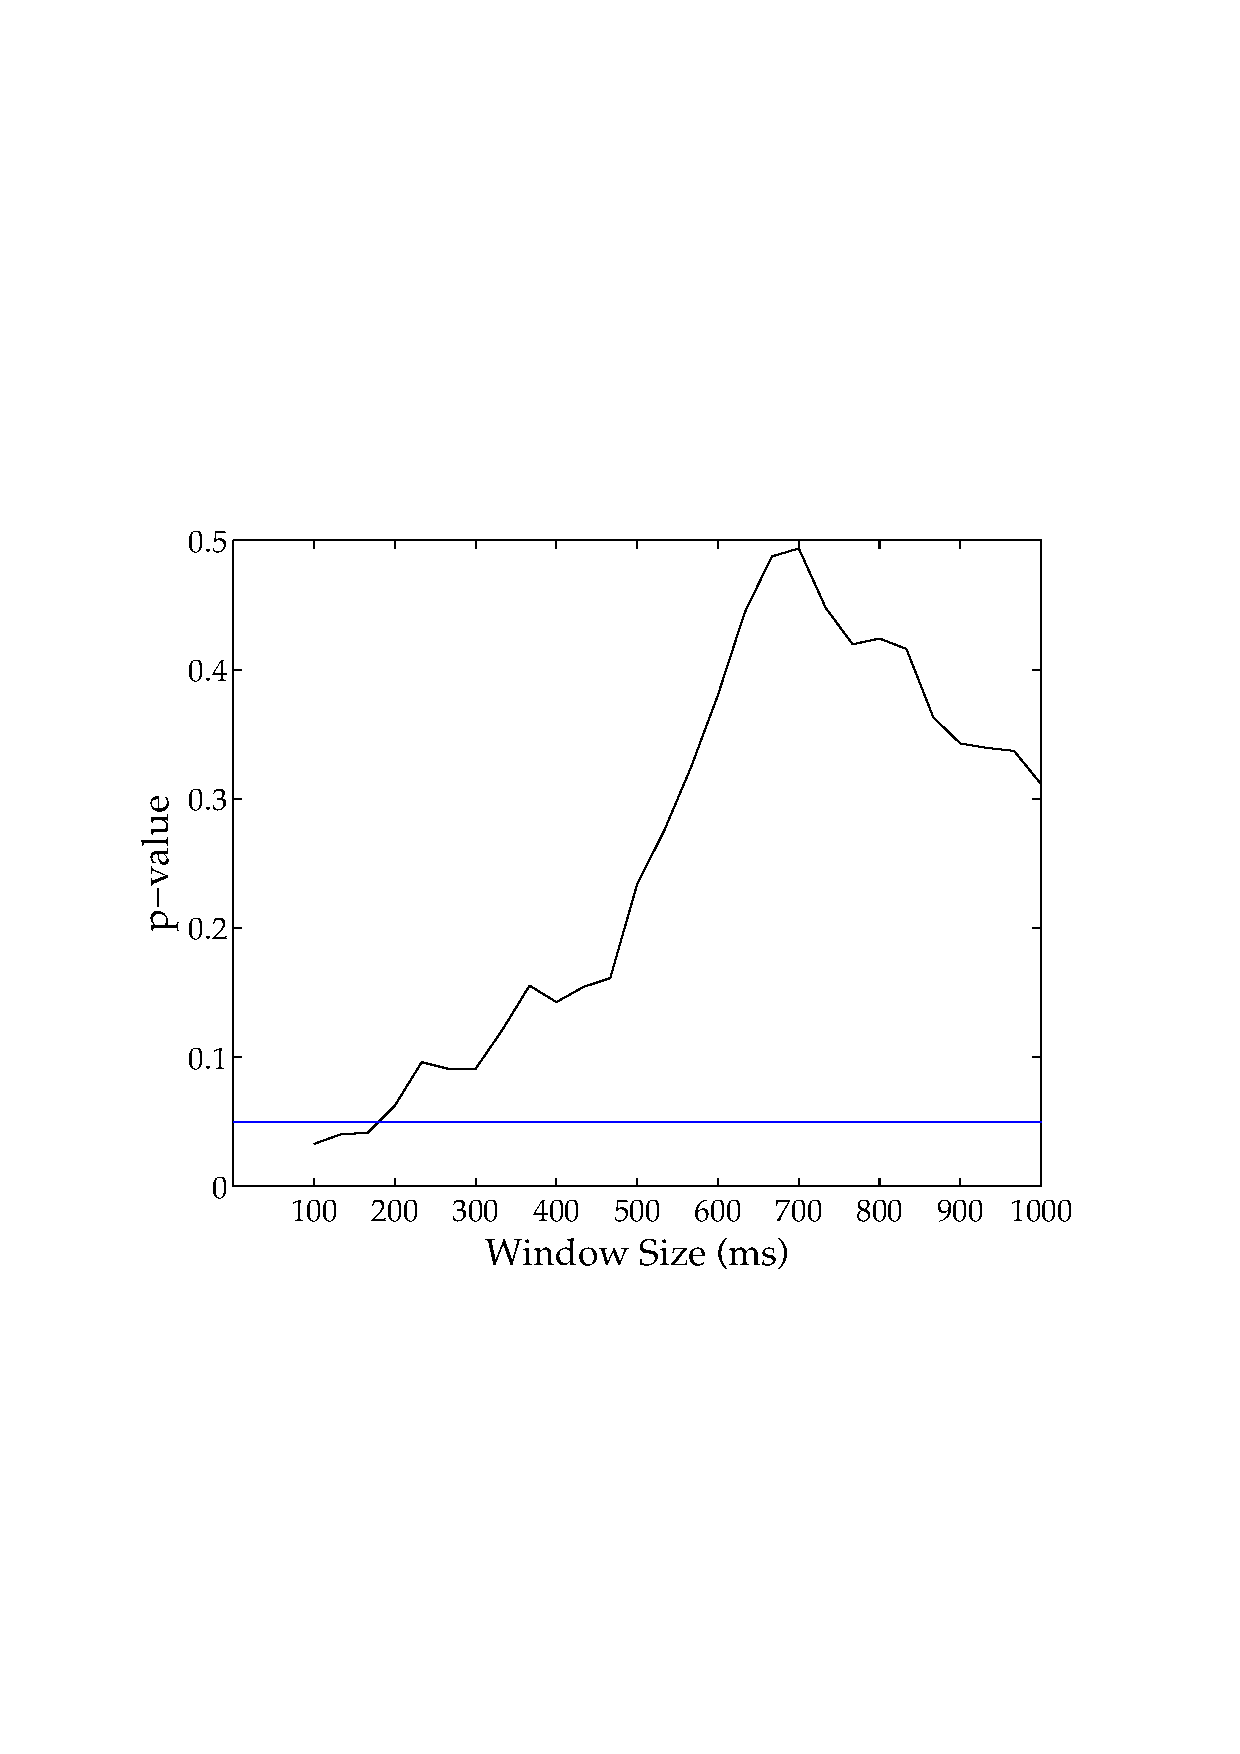
\includegraphics[width=70mm,height=64mm,trim=26mm 85mm 26mm 85mm]{./eps/gaze_var.pdf}}
  \caption[The significant levels of gaze variations with regard to the window sizes]{The significant levels of gaze variations with regard to the window sizes. The blue horizontal line shows the 5\% significant level.}
  \label{fig:gaze-variation}
\end{figure}

Using the saliency map from the computational bottom-up attention model, we examined the association between the gaze fitness to the model and the score. The fitness function is defined as below. We used the SaliencyToolbox with default parameters for getting the saliency map to analyze, and aligned the gaze coordination to the area of the saliency map, which had a smaller size after sub-sampling \cite{Walther2006}.

\begin{equation}\label{eq:salsum}
X_{saliency}^{(i,j)} = \sum_{t=1}^{T} \mathcal{S}_{x_{t},y_{t}}^{(i,j,t)}
\end{equation}

In Equation~\ref{eq:salsum}, $x_{t}$ and $y_{t}$ represent the mapped gaze coordination at $t$ time in a fixation duration. $\mathcal{S}^{(i,j,t)}$ is a saliency map which is the output of the model for a given screenshot at $t$ time in the duration of a movie clip, that was given to the participant $i$ for the $j$-th movie clip of the recognition test.

We fit the parameters for the linear regression model for the scores, which was defined by Equation~\ref{eq:lm},

\begin{equation}\label{eq:lm}
Y_{score} = \mathcal{B}_{0} + \sum_{l \in \mathcal{L}} \mathcal{B}_{l} \cdot X_{l}
\end{equation}

\noindent, $\mathcal{B}$s are the coefficients of the model, and $\mathcal{L}$ is a set of features as  

\begin{equation}\label{eq:l}
\mathcal{L} = \{duration, saliency\}.
\end{equation}

$X_{duration}$ is the fixation duration in second, and $X_{saliency}$ is defined by Equation~\ref{eq:salsum}. We used only the data of the long fixations, because the short fixated movie clips did not show the significant differences on the scores for the duration and the gaze fitness to the saliency map.

\begin{table}[ht]
\begin{center} 
\caption[Estimated coefficients of the linear regression model]{Estimated coefficients of the linear regression model.}
\vskip 0.12in
\label{tab:lr-coef} 
\begin{tabular}{lllll} 
\hline
Coef. & Estimate & SE & tStat & pValue \\ 
\hline
$\mathcal{B}_{0}$    &  4.8241   &  0.48622  &  9.9217 &  7.39e-16  \\
$\mathcal{B}_{duration}$ & -0.42214  &  0.18627  & -2.2663 &  0.025974    \\
$\mathcal{B}_{saliency}$ &  0.032642 &  0.015957 &  2.0455 &  0.043893    \\
\hline
\end{tabular} 
\end{center} 
\end{table}

Table~\ref{tab:lr-coef} shows the estimated coefficients of the linear regression model for the prediction. All shown parameters were statistically significant, though the gaze variation was excluded for the fitting due to its unexplainable for the scores. Whereas, the gaze fitness reasonably explained the score with the p-value 0.043893. The estimated value for the gaze fitness was positive, which means the score positively correlated with the gaze fitness in the model. Figure~\ref{fig:probing} shows a series of saliency probing for the gaze fitness. For details, please refer to the caption of that.

\begin{figure}
  \centerline{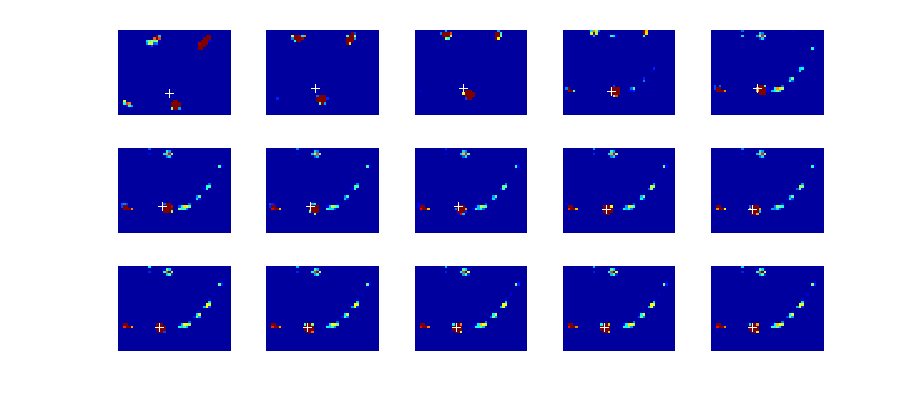
\includegraphics[width=86mm]{./eps/probing.png}}
  \caption[A series of saliency probing]{A series of saliency probing, one of those got the highest recognition score, is shown. From the left to the right, and from the top to the bottom, time goes with an interval of 100 ms (total length = 1500 ms). Each box represents a saliency map, the more reddish represents the higher saliency and the more bluish represents the lower saliency. The white cross represents the gaze position of the participant. As time goes, the eye gaze tracks down the highest saliency point (first row) and moves slowly in accordance with shifting of saliency map due to displacement of scene camera (second and third rows).}
  \label{fig:probing}
\end{figure}

Interestingly, the fixation duration, which was longer than 1400 ms, negatively correlated with the score, though the standard error of that was relatively high. 

The assessment of the model is shown in Table~\ref{tab:lr-goodness}. The number of observation was 88 since each of 11 participants rates 8 long fixated movie clips, respectively. The other models, like logistic regression and non-linear regression, are also examined, but they did not explain better than the linear model.

\begin{table}[ht]
\begin{center} 
\caption{Assessment of the linear regression model.} 
\vskip 0.12in
\label{tab:lr-goodness} 
\begin{tabular}{ll} 
\hline
Attribute   & Value \\ 
\hline
\# of observations & 88 \\
Error degree of freedom & 85 \\
RMSE & 1.34 \\
$R^{2}$ & 0.106 \\
Adjusted $R^{2}$ & 0.0847 \\
F-statistics vs. constant model & 5.02 (p-value = 0.00866) \\
\hline
\end{tabular} 
\end{center} 
\end{table}

\section{Discussions}

After all, what is the meaning of the long fixation durations on the video stimuli? Despite the fact that it could be a latency time to process the cognitive information of the visual stimuli, in the other perspective, it could be waiting time to the potentially salient moment on that eye position. The waiting on the prospective location for a dramatic change or a new event is an efficient way of information processing.

Though the long fixation itself does not describe the presence of the cognitive process to memorize, in the condition of the long fixation, the arousal effect is remarkable compared to the others in the condition of the short fixation. The short fixation is relatively complex and vague, the arousal effect on the short fixation might be not observable.

The characteristics of the eye movement on the arousal effect are probed by the statistical method and the computational attention model. First of all, as we report in Section~\nameref{subsec:gaze-variations}, the gaze variation on the alerted movie clips is smaller than those on the other case, when the window size is shorter than 200 ms, to minimize the variation from the slow pursuit. Yet, the gaze variation does not have a statistical power to predict on the recognition score, which is the measurement for the long-term memory. We conclude that the gaze variation partly explains only for the arousal effect, not for the further cognitive process, memorization.

Second, we establish the linear model to predict the score using the computational attention model in addition to the fixation duration. For the short fixated movie clips, we cannot find the predicting variables, so, only the observed data of the long fixated movie clips are used. This is the backward study of Itti (2006)’s work \cite{Itti2006}, which investigates the fitness of the model to human gaze, whereas our study uses the model to evaluate the attentiveness of human. In machine learning, Zou et al. (2012) reported that stimulated fixations help to capture the useful invariant features in the image recognition task \cite{Zou2012}. This gives a hint that how it works from a computational perspective.

Although we formulate the simple method via summation of saliency scores, the method shows the significant level for the prediction. The representation of saliency map is also found in the neuronal structures \cite{Fecteau2006}, which have a peak activity in the physically salient position. And, for the fixation durations longer than 1400 ms, the longer fixated movie clips are the lesser recognized. This suggests that the power of saliency probing tends to diminish as the fixation duration is behind time.

The value of the adjusted $R^{2}$ for the model reminds that the information of eye movement should be carefully used to estimate the cognitive process. There is the limitation of the analysis coverage, because the majority of the eye movement is the short fixated ones. 

Therefore, the investigation is not complete. We look forward to having more distinct features. A temporal modeling using the salient detectors \cite{marr1980,canny1986} and the optic flow \cite{koenderink1986} may be a promising option. Moreover, the cognitive modeling for the scene comprehension, which is related to the emotion-based reaction, guides us into the diffent level of a methodological stage. 

As discussed, the long fixations are constrained by the visual content of the video stimuli, and with regard to that, the eye movements are planned in a reciprocal manner \cite{zhang2013}. The estimation of the eye movement is viable on top of a reciprocally anticipatory model \cite{robert1985anticipatory}. The serial information of the fixation positions can be used to parsimoniously select the portion of visual features on the scene for an application using the features, and, it can be a methodological breakthrough for the cognitive modeling on the endless stream of the visual information.


\section{Conclusions}

The visual constraints, which induce long fixations, are summed up as three distinctive types: alerted, successive and stationary. We found the arousal effect only for the long fixated movie clips of the alerted type. The small gaze variation for the long fixation indicates an active response to the arousal stimuli. Though, the gaze variation does not help to estimate for the recognition score, among long fixations, fixation duration and saliency-probing activity are significant for that. We can appreciate this computational model within the embodied cognitive framework with the perception-action cycling.


\section{Acknowledgments}

This work was supported by the National Research Foundation of Korea (NRF) grant funded by the Korea government (MSIP) (NRF-2010-0017734-Videome),
supported in part by ICT R\&D program funded by the Korea government (MSIP/IITP) (10035348-mLife, 14-824-09-014, 10044009-HRI.MESSI).

\bibliographystyle{apacite}

\setlength{\bibleftmargin}{.125in}
\setlength{\bibindent}{-\bibleftmargin}

\bibliography{kim2015activelong}

\end{document}
